\chapter{Planificación}
\label{chap:planification}


\section{Fases}

La planificación del desarrollo del proyecto se ha dividido en las fases que vamos a ver a continuación.

\subsection{Fase inicial}

En esta etapa es donde se definen las bases del proyecto. Se expone la motivación que nos conduce a llevar el proyecto a cabo, se identifican las necesidades y se establecen unos objetivos principales que deberán de cumplirse a lo largo del desarrollo del proyecto. Esta información podemos verla en el capítulo 1 (\hyperref[chap:introduction]{ver página}) de este documento. 

\subsection{Fase de investigación}

Durante esta fase, se recopila información para entender el entorno donde se pondrá en práctica la aplicación. Para ello, se investigarán cuestiones como la definición de negocio minorista, un estudio de los pequeños negocios mixtos y un estudio de los comerciantes minoristas. Además, con el objetivo de que la aplicación cumpla los términos legales, también se realizará un estudio sobre usabilidad, accesibilidad y la legislación de protección de datos. 

Para finalizar esta fase de investigación y entender la verdadera necesidad de desarrollar esta aplicación, se realizará una comparación de aplicaciones similares en el mercado. 

\subsection{Fase de análisis}

En esta fase encontraremos 2 apartados: 

\begin{itemize}
	\item \textbf{Análisis de las tecnologías:} En este apartado encontraremos una lista de las tecnologías que se han utilizado para el desarrollo del proyecto, además de una explicación de porqué han sido seleccionadas y cuáles son sus principales características.  
	\item \textbf{Análisis de la aplicación:} Durante este aparado se estudian los requisitos que deberá de cumplir la aplicación para satisfacer las necesidades del cliente. Para una mayor especificación y claridad, se desarrollarán los casos de uso y los diagramas de secuencia del sistema. Para entender como se relacionan las entidades, también se hará un modelo conceptual. 
\end{itemize}


\subsection{Fase de diseño}

En esta fase, se especifica más en detalle cómo va a construirse la aplicación mediante un diagrama de la arquitectura del sistema y los bocetos de la interfaz gráfica del usuario. Los bocetos se harán pantalla a pantalla y organizados por los mismos grupos que los requisitos para una mayor claridad. 


\subsection{Fase de desarrollo}

Esta es la fase donde se construye el producto que hemos definido en la fase de análisis y diseño. Será la etapa más larga ya que se transforman todos los planes y diseños previos en código, dando como resultado un entregable final funcional.\\

Esta fase se dividirá en tres iteraciones, ya que la metodología utilizada para la implementación de la aplicación es una metodología ágil. En cada iteración se escogerá el alcance de la iteración, es decir, los requisitos que se van a llevar a cabo, se realizará la implementación de estos, se testeará y se le expondrá al usuario para que pueda validarlo. Con la validación de usuario se obtendrá información de mejoras que deberán de ser aplicadas en las siguientes iteraciones. 

Tras finalizar las tres iteraciones, se obtendrá un entregable final funcional que se le proporcionará al cliente para que pueda disfrutar de este. 


\subsection{Redacción de la memoria}

Con el objetivo de documentar el desarrollo del proyecto, se va a plasmar toda la información relevante en este documento. No se ha incluido en ninguna fase ya que la documentación se irá haciendo a lo largo de todo el desarrollo del proyecto. 

\subsection{Diagrama de Gantt}

En la siguiente tabla podemos ver cuál ha sido la duración en horas de cada una de las tareas que se exponen en el diagrama de Gantt. El diagrama representa la planificación temporal de las tareas del proyecto. Cada celda representa una semana del mes. En la tabla se muestran las horas y en el diagrama el momento en el que se realizó. 

\begin{table}[h!]
	\centering
	\begin{tabular}{|l|c|}
		\hline
		\textbf{Fase} & \textbf{Horas} \\ \hline
		Motivación & 2 \\ \hline
		Objetivos del proyecto & 3 \\ \hline
		Estructura del documento & 2 \\ \hline
		Definición de un negocio minorista & 10 \\ \hline
		Estudio de los pequeños negocios mixtos & 10 \\ \hline
		Estudio de comerciantes minoristas & 10 \\ \hline
		Estudio de usabilidad y accesibilidad & 12 \\ \hline
		Legislación actual de protección de datos & 5 \\ \hline
		Aplicaciones similares y comparativas & 15 \\ \hline
		Análisis de tecnologías a utilizar & 10 \\ \hline
		Especificación de requisitos & 15 \\ \hline
		Modelos de casos de uso & 20 \\ \hline
		Modelo conceptual & 3 \\ \hline
		Modelos de comportamiento & 20 \\ \hline
		Diagrama de arquitectura del sistema & 1 \\ \hline
		Diseño de la interfaz gráfica & 10 \\ \hline
		Primera iteración & 40 \\ \hline
		Segunda iteración & 45 \\ \hline
		Tercera iteración & 30 \\ \hline
		Creación y modificaciones de la base de datos & 15 \\ \hline
		Redacción de la memoria & 40 \\ \hline
		\textbf{Total} & \textbf{308} \\ \hline
	\end{tabular}
	\caption{Distribución de horas por fase}
	\label{tabla:resumen}
\end{table}



\newpage

\begin{figure}[H]
	\centering
	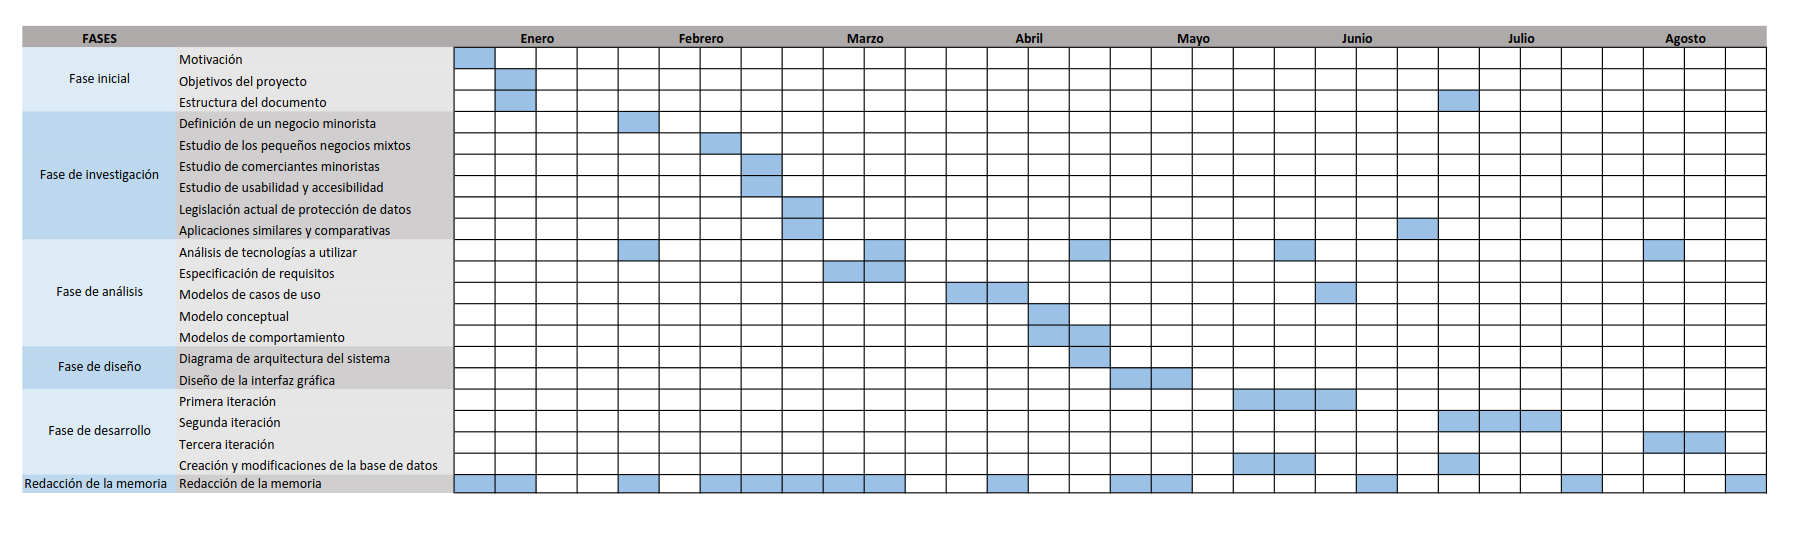
\includegraphics[width=1.6\textwidth, angle=90]{imagenes/imagenesDiagramas/diagramaGantt.png}
	\caption{Diagrama de Gantt}
	\label{fig:diagramaGantt}
\end{figure}



\newpage

\section{Presupuesto}

\subsection{Recursos}

En este apartado se va a exponer los recursos hardware y software que se van a utilizar para el desarrollo del proyecto. 

\begin{adjustwidth}{2em}{0pt} % Aumenta el margen izquierdo por 2em
\subsubsection{Hardware}

Los componentes hardware que se van a utilizar para llevar a cabo el proyecto son: 

\begin{itemize}
	\item \textbf{Ordenador:} MSI Prestige 15 A10SC.
\end{itemize}

\subsubsection{Software}

Las herramientas software que se van a utilizar para llevar a cabo el proyecto son: 

\begin{itemize}
	\item \textbf{Sistema Operativo:} Ubuntu 20.04
	\item \textbf{Lenguaje de programación:} Flutter
	\item \textbf{IDE:} Visual Studio Code
	\item \textbf{Diseño de diagramas UML:} Visual Paradigm
	\item \textbf{Sistema de composición de texto:} LaTeX
	\item \textbf{Editor de texto:} TeXstudio
\end{itemize}
\end{adjustwidth} 

\subsection{Costes}

En esta sección vamos a analizar el coste total del proyecto. Vamos a distinguir distintos apartados. 

\begin{adjustwidth}{2em}{0pt} % Aumenta el margen izquierdo por 2em
	\subsubsection{Licencias}
	
	Un tipo de coste que conlleva el desarrollo de un proyecto es la adquisición de las licencias necesarias para la producción del mismo. Las licencias que se van a utilizar en este proyecto son de software libre y por tanto son gratuitas. Esto significa que no supondrán ningún coste adicional. Las licencias que se utilizarán son las siguientes: 

\newpage

	\begin{itemize}
		\item \textbf{Ubuntu 20.04:} GNU General Public Licence (GPL).
		\item \textbf{Flutter:} Licencia BSD. 
		\item \textbf{Visual Paradigm:} Licencia adquirida por usos académicos. 
		\item \textbf{LaTeX:} LaTeX Project Public License (LPPL).
	\end{itemize}
	
	
	\subsubsection{Recursos materiales}
	
	El único recurso material que se va utilizar para el desarrollo del proyecto es el ordenador personal. \\
	
	El periodo de amortización común para los ordenadores y equipos informáticos es de 3 a 5 años. Realizaremos la media y utilizaremos un periodo de 4 años para los cálculos. Sabiendo que el equipo costó 1400€, se amortizará 350€ al año. Como la duración del proyecto es de 5 meses, el coste final de los recursos materiales será de 145'83€
	
	\subsubsection{Recursos humanos}
	
	En esta sección se incluyen los gastos por la contratación de personal. Este proyecto solamente lo va a desarrollar una persona, bajo la titulación de programador senior. \\
	
	En la actualidad, un programador senior recibe una media de 22.000€ anuales. Durante los 5 meses que dura el proyecto, se estima un salario de 9166'66€. 
	
	\subsubsection{Otros}
	
	Este apartado engloba costes indirectos como los gastos debidos a la localización para trabajar, los gastos de transporte, conexión a Internet, etc. Este gasto se suele aproximar a un 10\% de los gastos de recursos humanos. Por tanto, la cantidad estipulada para este apartado sería de 916'66€. 
	
	\newpage
	
	\subsubsection{Total}
	
% Tabla presupuesto total
\begin{table}[htb!]
	\centering % Centra la tabla en la página
	\begin{tabular}{|p{0.3\linewidth}|p{0.35\linewidth}|p{0.35\linewidth}|}
		\hline
		\rowcolor{grayshade} \textbf{Descripción} & \textbf{Coste mensual} & \textbf{Coste total} \\
		\hline
		\textbf{Licencias} & 0€ & 0€ \\
		\hline
		\textbf{Recursos materiales} & 29'17€ & 145'83€ \\
		\hline
		\textbf{Recursos humanos} & 1833'33€ & 9166'66€ \\
		\hline
		\textbf{Otros} & 183'33€ & 916'66€ \\
		\hline
		\textbf{Total} & 2045,83€ & 10.229'15€ \\
		\hline
	\end{tabular}
	\caption{Presupuesto total}
\end{table}
\end{adjustwidth} 
